\chapter{Desarrollo del Proyecto}

\minitoc

\section{Introducción}

\begin{figure}[!tb]
	\centering
	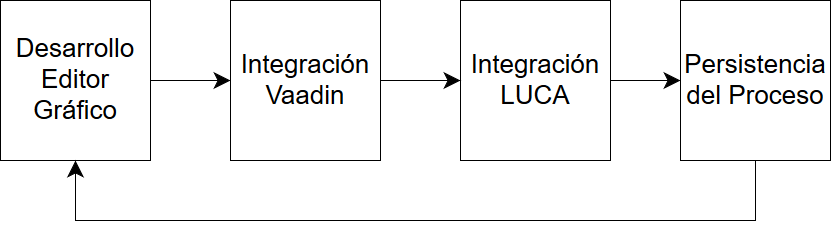
\includegraphics[width=\linewidth]{flujoDesarrollo.png}
	\caption{Flujo de Desarrollo}
	\label{fig:flujoDesarrollo}
\end{figure}

%% Decir qué cuenta esta sección y los pasos generales que se han dado para
%% desarrollar el \emph{Process Editor}

El presente capítulo detalla el proceso de desarrollo del proyecto realizado dentro de este Trabajo Fin de Grado. Tal como se ha comentado, el objetivo del proyecto era 
proporciona al producto LUCA una herramienta gráfica para poder crear \emph{procesos}, es decir, poder encadenar consultas entre sí a raíz de sus valores de entrada y de salida.

Para alcanzar este objetivo, se siguió el esquema de trabajo que se muestra en la Figura~\ref{fig:flujoDesarrollo}.  

La primera etapa consistió en realizar un primer contacto con la herramienta \emph{GoJS}, para ello, se realizó una prueba de concepto donde se creaba un diagrama sencillo con cajas o nodos que se conectan entre sí (Figura~\ref{}).

Con la prueba de concepto funcionando, la siguiente etapa consistió en integrar el diagrama en \emph{GoJS} con el framework de \emph{Vaadin} para obtener un proyecto implementado en \emph{Java} que pueda ser utilizado por otro proyectos.

La tercera etapa se centró en integrar dicho proyecto \emph{Vaadin} antes mencionado en el producto LUCA con el objetivo de ser capaces de mostrar el editor y ser capaces de interactuar con él y recibir los eventos ocurridos.

Por último, la cuarta etapa consistió en añadir la capa de negocio y de persistencia al modelo de datos de LUCA, creado específicamente para persistir \emph{procesos} y toda su jerarquía de clases.

Una vez acabadas las cuatro etapas de desarrollo, comenzó un curso de iteraciones para refinar el proyecto e ir dando la complejidad final al mismo, de forma que se fue completando toda la lógica de negocio, así como, el aspecto gráfico final.

Las siguientes secciones proporcionan detalles sobre la ejecución de cada etapa.

\section{Desarrollo del Editor Gráfico}

%% Describir los pasos, a nivel general, para crear el editor gráfico sencillo. 

%% Añadir algo de código. 


%% Qué se hizo en otras iteraciones, a modo de la lista de la compra (y teniendo en 
%%    cuenta que son cosas gráficas)

%% Código de aquello en lo que te quieras lucir (opcional)

%% Hablar algo de pruebas. 

\section{Integración del editor con \emph{Vaadin}}

%% Explicar que necesitamos hacer que los eventos del editor se redirijan a Vaadin
El objetivo principal del editor gráfico de \emph{procesos} es proporcionar una interfaz, con la que otros proyectos que quieran utilizar este editor se puedan comunicar para poder gestionar los \emph{procesos}.

%% Explicar que la redirección se hace mediante un conector en Javascript
Para ello es necesario que exista una comunicación entre la herramienta \emph{GoJS} y \emph{Vaadin} mediante eventos. Estos eventos producidos en \emph{GoJS} son trasladados al proyecto \emph{Vaadin}, para que sean comunicados al proyecto que utilice este componente gráfico (en nuestro caso, este papel lo ocupara el producto de LUCA, que deberá decidir que eventos escuchar y como reaccionar ante ellos).

Para que esta comunicación entre \emph{GoJS} y \emph{Vaadin} sea posible, es necesario un fichero que realice las funciones de conector (a partir de ahora lo llamaremos \emph{conector}), su objetivo será comunicar a \emph{Vaadin} de los eventos ocurrido en el editor gráfico y, siguiendo las órdenes de \emph{Vaadin} realizar cambios sobre la interfaz del editor gráfico. De esta forma se produce un diálogo entre ambos conceptos en base a eventos y cambios en la interfaz gráfica.


%% Mostrar un trozo de código del conector muy sencillo

%% Explicar que en algunos casos fue necesario alterar el flujo de funcionamiento 
%% normal de GoJS y describir el caso del link.
En algunas ocasiones fue necesaria  modificar el comportamiento interno de algunas funciones de \emph{GoJS}, por ejemplo, cuando se realiza una conexión a nivel gráfico, en el modelo de \emph{GoJS} se instancia un enlace, sin embargo, debido a que no se requería de dicha funcional (sino que lo que se quería era solo mandar el evento de enlazado, para después, si era necesario enlazar), fue necesario sobreescribir dicha funcionalidad para evitar que se produzca dicha instanciación (Figura~\ref{}).

%% Explicar figura del link

%% Hablar algo de pruebas. 
Debido a la complejidad que existe para comprobar que las acciones que se realizan desde el proyecto del editor a nivel \emph{Java} se muestran gráficamente en el editor, no se han realizado pruebas automatizadas, aunque si se realizaron pruebas o verificaciones del funcionamiento visualmente en base a las acciones que se pueden realizar sobre el mismo, como son la creación de procesos y enlazado entre ellos.


\section{Integración del editor con LUCA}

%% Decribir los pasos, a nivel general, para integrar el editor básico. 

%% Mostrar captura de la interfaz

%% Qué se hizo en otras iteraciones, a modo de la lista de la compra.

%% Mostrar código de algo no trivial 

%% Hablar algo de pruebas. 

\section{Gestión y Persistencia de los Procesos}

El objetivo de este paso era que LUCA pudiese almacenar y gestionar procesos. Para ello lo primero era definir un modelo conceptual de datos para los procesos. Dicho modelo conceptual se muestra en la Figura~\ref{}.

%% Explicar que ese modelo concetual de datos se implementa en Java y con JPA se 
%% genera el esquema relacional y el puente objeto-relacional.

%% Indicar qué ha sido necesario modificar en la capa de negocio (control de accesos)
%% y negocio (servicio). Mostrar ejemplos de código

%% Qué se hizo en otras iteraciones, a modo de la lista de la compra.

%% Hablar algo de pruebas, y si las hay, mostrar código.
